\subsection{Cyclopentyl alcohol derivatives}

\subsubsection{Head-group synthesis}

\begin{scheme}[H]
	\begin{center}
		\schemeref[Ocy5]{cmpd:Ocy5}
		\schemeref[NH2MeBn]{cmpd:NH2MeBn}
		\schemeref[HOcy5NHMeBn_RRS]{cmpd:HOcy5NHMeBn_RRS}
		\schemeref[HOcy5NHMeBn_SSS]{cmpd:HOcy5NHMeBn_SSS}
		\schemeref[HOcy5NH2_RR]{cmpd:HOcy5NH2_RR}
		\schemeref[HOcy5NH2_SS]{cmpd:HOcy5NH2_SS}
		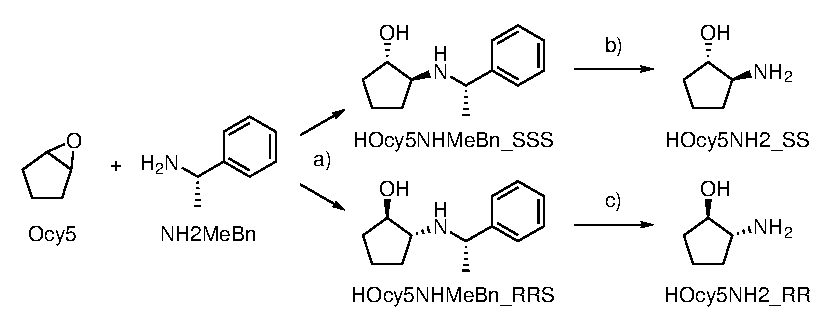
\includegraphics[scale=1]{HOcy5NH2_synth}
		\caption{
		a) \ce{AlMe3}, \ce{CH2Cl2}, 0 $^\circ$C. \compound{cmpd:HOcy5NHMeBn_SSS} : 32.1 \%, \compound{cmpd:HOcy5NHMeBn_RRS} : 35.2 \%.
		b) \ce{Pd(OH)2}, MeOH, \ce{H2}, 5 atm, r.t., 1 d, \compound{cmpd:HOcy5NH2_RR} : 100 \%, \compound{cmpd:HOcy5NH2_RR} : 100 \%.
		\label{sch:HOcy5NH2_synth}}
	\end{center}
\end{scheme}

\subsubsection{Initial branching strategy}

\begin{scheme}[H]
	\begin{center}
		\schemeref[HOcy5NH2]{cmpd:HOcy5NH2_SS}
		\schemeref[HOcy5NH4Br]{cmpd:HOcy5NH4Br_SS}
		\schemeref[HOcy5NH4N3]{cmpd:HOcy5NH4N3_SS}
		\schemeref[HOcy5NH4CipMe]{cmpd:HOcy5NH4CipMe_SS}
		\schemeref[HOcy5NH4T4Cip]{cmpd:HOcy5NH4T4Cip_SS}
		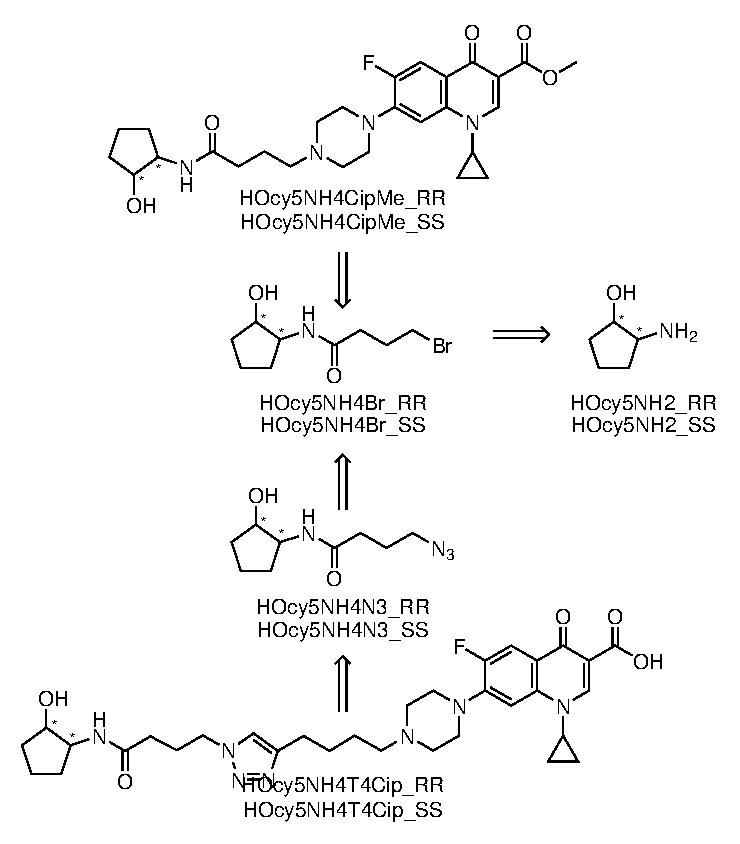
\includegraphics[scale=1]{HOcy5NH4_retro_A}
		\caption{\label{sch:HOcy5NH4_retro_A}}
	\end{center}
\end{scheme}

Failed. Lots of side-products.

%LMO-2-058

\begin{scheme}[H]
	\begin{center}
		\schemeref[HOcy5NH2]{cmpd:HOcy5NH2_SS}
		\schemeref[Cl4Br]{cmpd:Cl4Br}
		\schemeref[HOcy5NH4Br]{cmpd:HOcy5NH4Br_SS}
		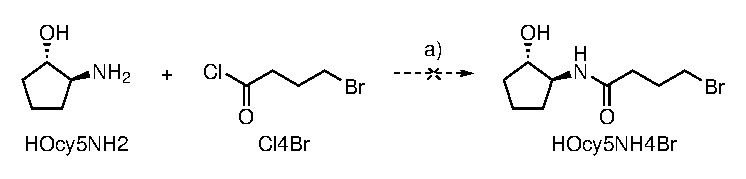
\includegraphics[scale=1]{HOcy5NH4Br_SS_synth}
		\caption{\label{sch:HOcy5NH4Br_SS_synth}}
	\end{center}
\end{scheme}

\subsubsection{TBS protection strategy}

\subsubsubsection{Initial}

\begin{scheme}[H]
	\begin{center}
		\schemeref[HOcy5NH2]{cmpd:HOcy5NH2_SS}
		\schemeref[TBSOcy5NH2]{cmpd:TBSOcy5NH2_SS}
		\schemeref[TBSOcy5NH4Br]{cmpd:TBSOcy5NH4Br_SS}
		\schemeref[TBSOcy5NH4N3]{cmpd:TBSOcy5NH4N3_SS}
		\schemeref[TBSOcy5NH4CipMe]{cmpd:TBSOcy5NH4CipMe_SS}
		\schemeref[TBSOcy5NH4T4Cip]{cmpd:TBSOcy5NH4T4Cip_SS}
		\schemeref[HOcy5NH4CipMe]{cmpd:HOcy5NH4CipMe_SS}
		\schemeref[HOcy5NH4T4Cip]{cmpd:HOcy5NH4T4Cip_SS}
		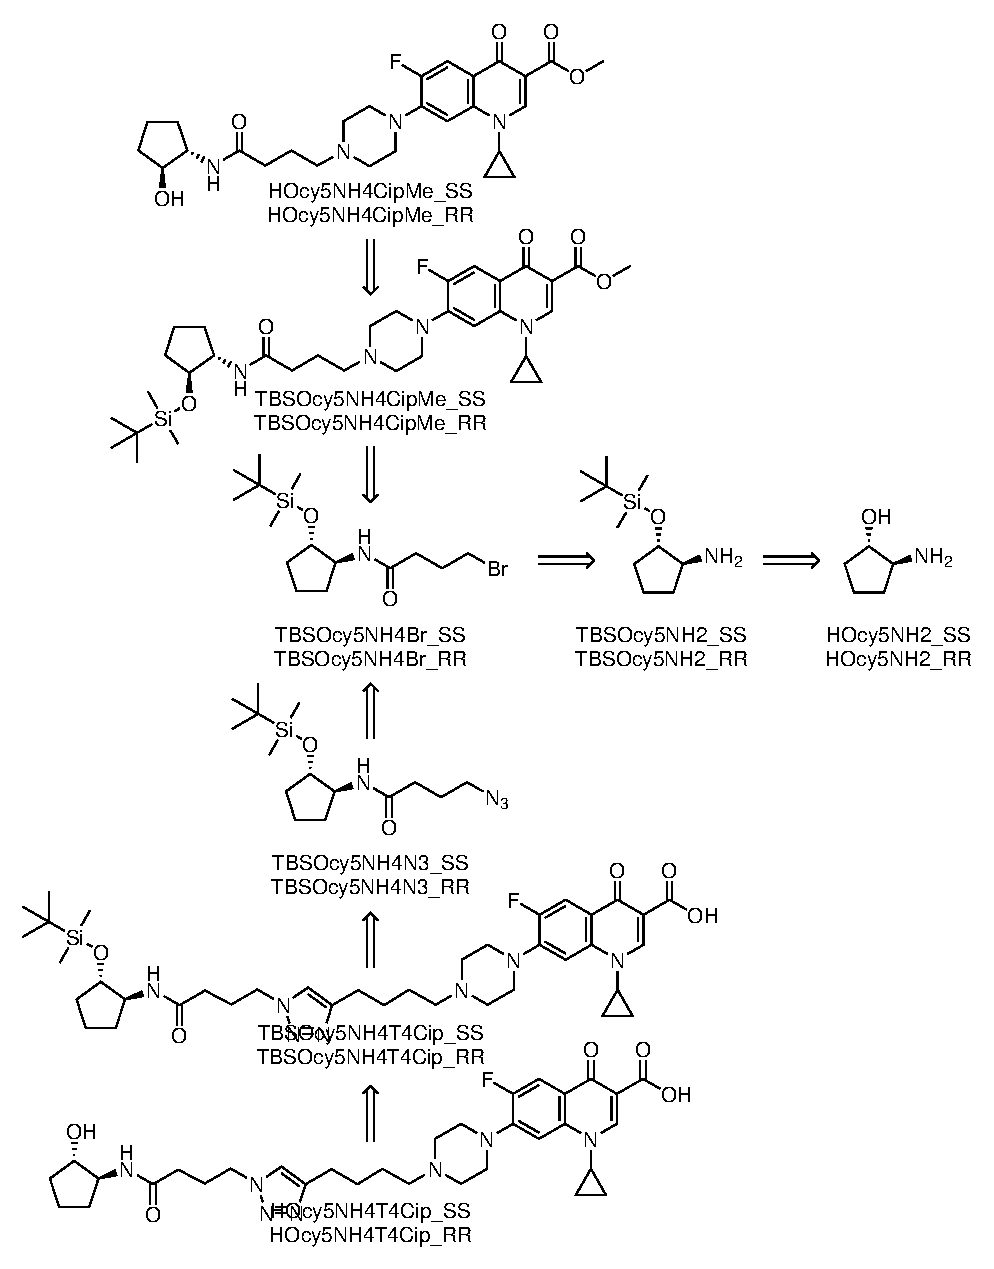
\includegraphics[scale=1]{HOcy5NH4_retro_B}
		\caption{\label{sch:HOcy5NH4_retro_B}}
	\end{center}
\end{scheme}

Want to protect alcohol to stop side reactions

\begin{scheme}[H]
	\begin{center}
		\schemeref[HOcy5NH2]{cmpd:HOcy5NH2_SS}
		\schemeref[TBSOcy5NH2]{cmpd:TBSOcy5NH2_SS}
		\schemeref[TBSOcy5NH4Br]{cmpd:TBSOcy5NH4Br_SS}
		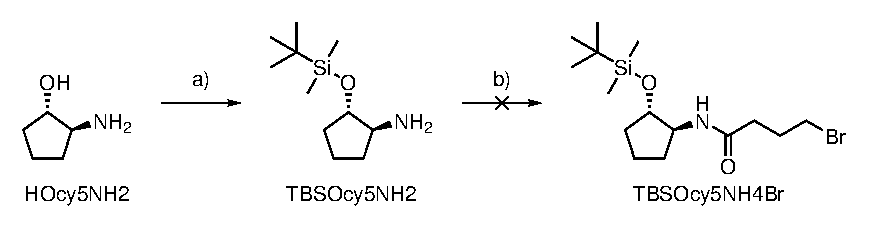
\includegraphics[scale=1]{TBSOcy5NH4Br_SS_synth}
		\caption{\label{sch:TBSOcy5NH4Br_SS_synth}}
	\end{center}
\end{scheme}

Protection optimisation

Still get side-reactions when adding tail

\subsubsubsection{Triazoles by two-step reaction}
Talk about moving to two-step reaction.

\begin{scheme}[H]
	\begin{center}
		\schemeref[TBSOcy5NH2]{cmpd:TBSOcy5NH2_SS}
		\schemeref[Cl4Br]{cmpd:Cl4Br}
		\schemeref[TBSOcy5NH4Br]{cmpd:TBSOcy5NH4Br_SS}		\schemeref[TBSOcy5NH4N3]{cmpd:TBSOcy5NH4N3_SS}
		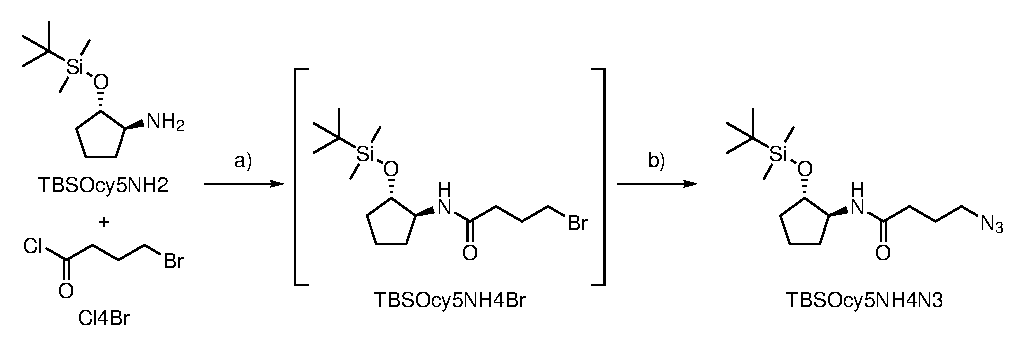
\includegraphics[scale=1]{TBSOcy5NH4N3_SS_synth_2step}
		\caption{\label{sch:TBSOcy5NH4N3_SS_synth_2step}}
	\end{center}
\end{scheme}

\begin{scheme}[H]
	\begin{center}
		\schemeref[TBSOcy5NH4N3]{cmpd:TBSOcy5NH4N3_SS}
		\schemeref[Y4Cip]{cmpd:Y4Cip}
		\schemeref[TBSOcy5NH4T4Cip]{cmpd:TBSOcy5NH4T4Cip_SS}
		\schemeref[HOcy5NH4T4Cip]{cmpd:HOcy5NH4T4Cip_SS}
		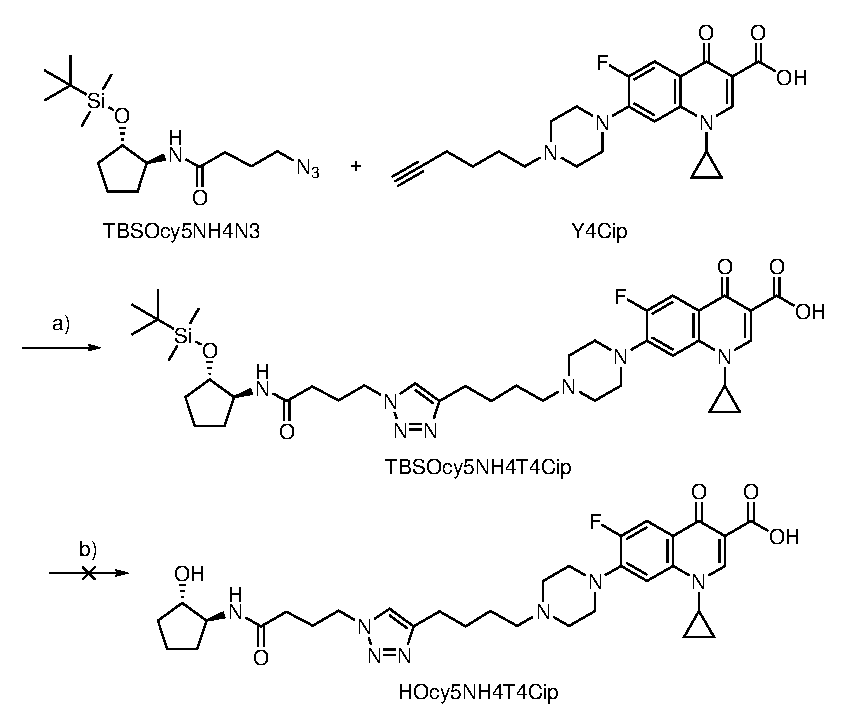
\includegraphics[scale=1]{TBSOcy5NH4T4Cip_SS_synth}
		\caption{\label{sch:TBSOcy5NH4T4Cip_SS_synth}}
	\end{center}
\end{scheme}

Did click, then failed to deprotect.

\subsubsection{Attaching the linker to ciprofloxacin first}

Given the side-reactions and low yields associated with the literate synthesis of the S$_N$2 conjugates proposed by Ganguly et. al\cite{Ganguly2011}, we investigated a second synthesis, building up the linker on the ciprofloxacin side before coupling with the head group (see \ref{sch:HOcy5NH4CipMeRR_synth}).

\begin{scheme}[H]
	\begin{center}
		\schemeref[HOcy5NH2]{cmpd:HOcy5NH2_SS}
		\schemeref[HOO4CipMe]{cmpd:HOO4CipMe}
		\schemeref[tBuOO4CipMe]{cmpd:tBuOO4CipMe}
		\schemeref[tBuOO4Br]{cmpd:tBuOO4Br}
		\schemeref[CipMe]{cmpd:CipMe}
		\schemeref[HOcy5NH4CipMe_SS]{cmpd:HOcy5NH4CipMe_SS}
		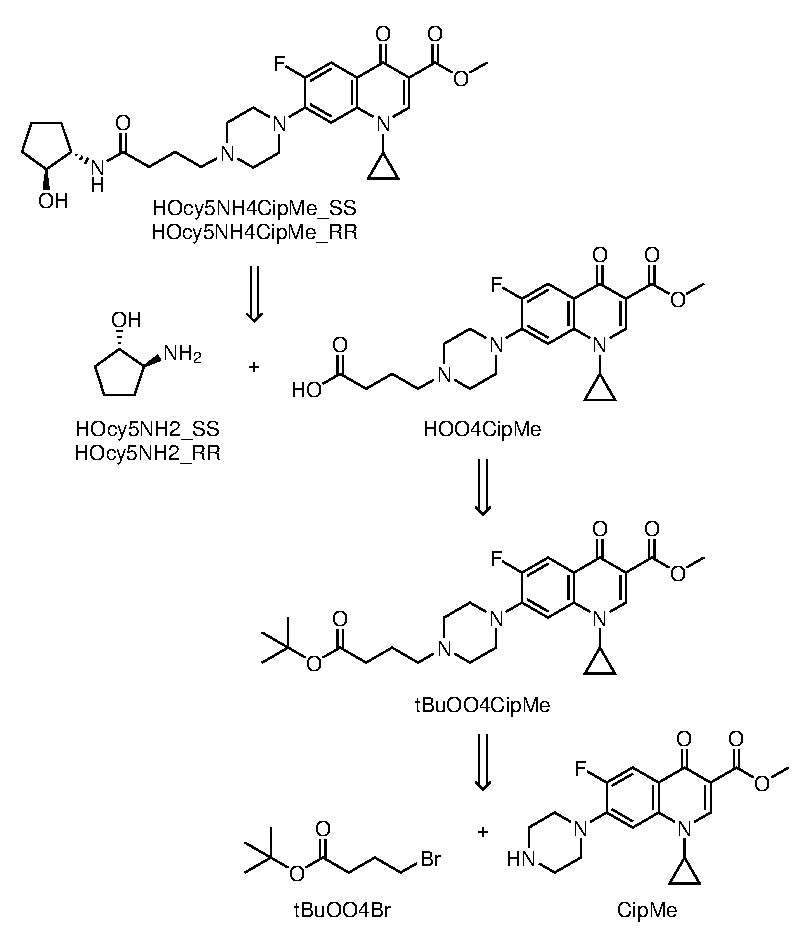
\includegraphics[scale=1]{HOcy5NH4_retro_D}
		\caption{\label{sch:HOcy5NH4_retro_D}}
	\end{center}
\end{scheme}

\subsubsubsection{Synthesis of methyl-protected ciprofloxacin with linker with terminal carboxylate}

\begin{scheme}[H]
	\begin{center}
		\schemeref[CipMe]{cmpd:CipMe}
		\schemeref[tBuOO4Br]{cmpd:tBuOO4Br}
		\schemeref[tBuOO4CipMe]{cmpd:tBuOO4CipMe}
		\schemeref[HOO4CipMe]{cmpd:HOO4CipMeTFA}
		\schemeref[HOcy5NH2]{cmpd:HOcy5NH2_SS}
		\schemeref[HOcy5NH4CipMe_SS]{cmpd:HOcy5NH4CipMe_SS}
		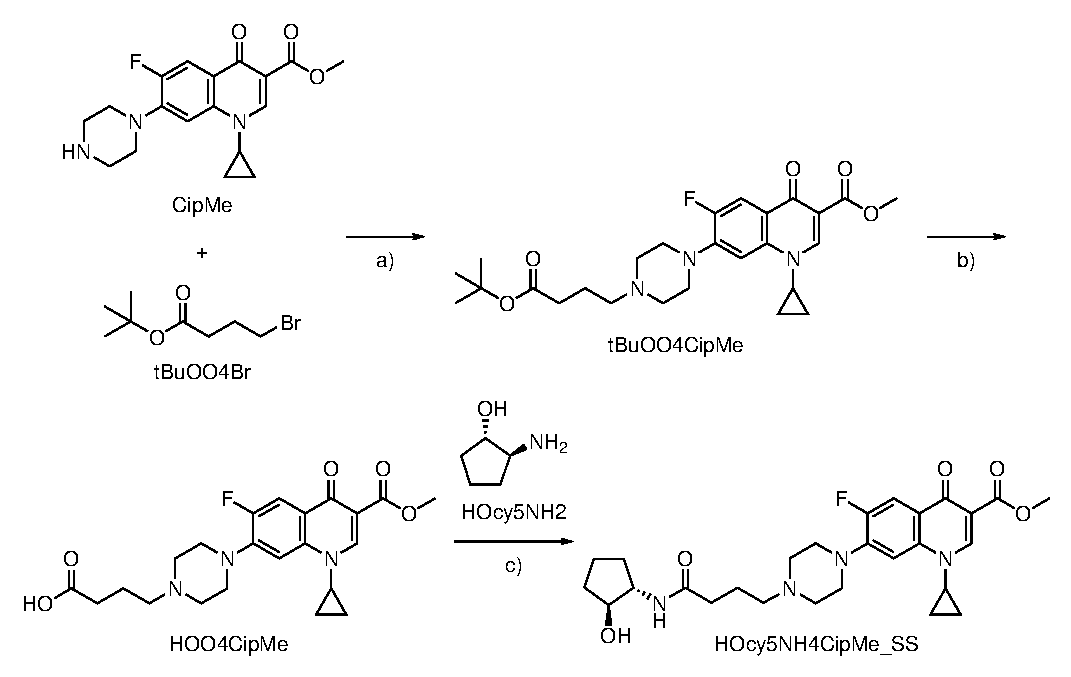
\includegraphics[scale=1]{HOcy5NH4CipMe_SS_synth}
		\caption{Synthesis of \compound{cmpd:HOcy5NH4CipMe_SS}. 
			a) . 
			\label{sch:HOcy5NH4CipMe_SS_synth}}
	\end{center}
\end{scheme}



\subsubsection{Triazoles from the chloride}

\begin{scheme}[H]
	\begin{center}
		\schemeref[HOcy5NH2]{cmpd:HOcy5NH2_SS}
		\schemeref[HOcy5NH4Cl]{cmpd:HOcy5NH4Cl_SS}
		\schemeref[HOcy5NH4N3]{cmpd:HOcy5NH4N3_SS}
		\schemeref[HOcy5NH4CipMe]{cmpd:HOcy5NH4CipMe_SS}
		\schemeref[HOcy5NH4T4Cip]{cmpd:HOcy5NH4T4Cip_SS}
		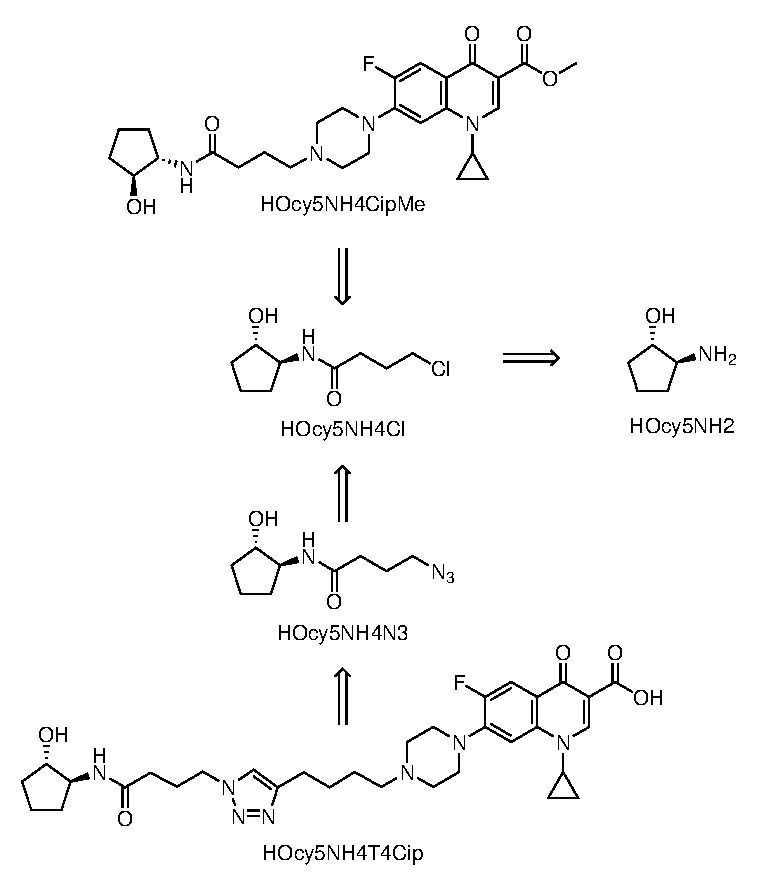
\includegraphics[scale=1]{HOcy5NH4_retro_C}
		\caption{\label{sch:HOcy5NH4_retro_C}}
	\end{center}
\end{scheme}

\begin{scheme}[H]
	\begin{center}
		\schemeref[HOcy5NH2]{cmpd:HOcy5NH2_SS}
		\schemeref[Cl4Cl]{cmpd:Cl4Cl}
		\schemeref[HOcy5NH4Cl]{cmpd:HOcy5NH4Cl_SS}
		\schemeref[HOcy5NH4N3]{cmpd:HOcy5NH4N3_SS}
		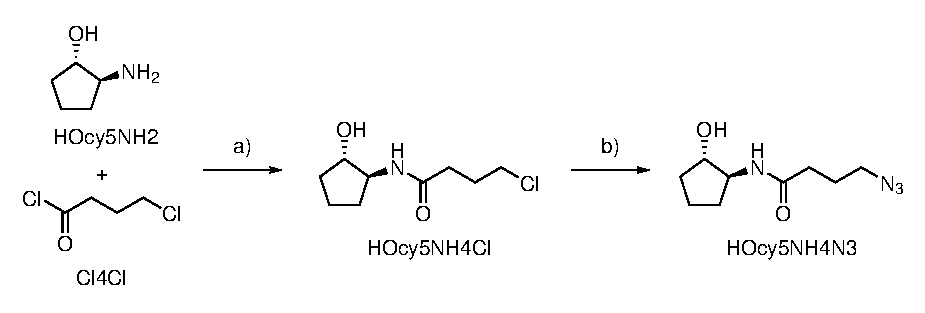
\includegraphics[scale=1]{HOcy5NH4N3_SS_synth}
		\caption{\label{sch:HOcy5NH4N3_SS_synth}}
	\end{center}
\end{scheme}

\begin{scheme}[H]
	\begin{center}
		\schemeref[HOcy5NH4N3]{cmpd:HOcy5NH4N3_SS}
		\schemeref[Y4Cip]{cmpd:Y4Cip}
		\schemeref[HOcy5NH4T4Cip]{cmpd:HOcy5NH4T4Cip_SS}
		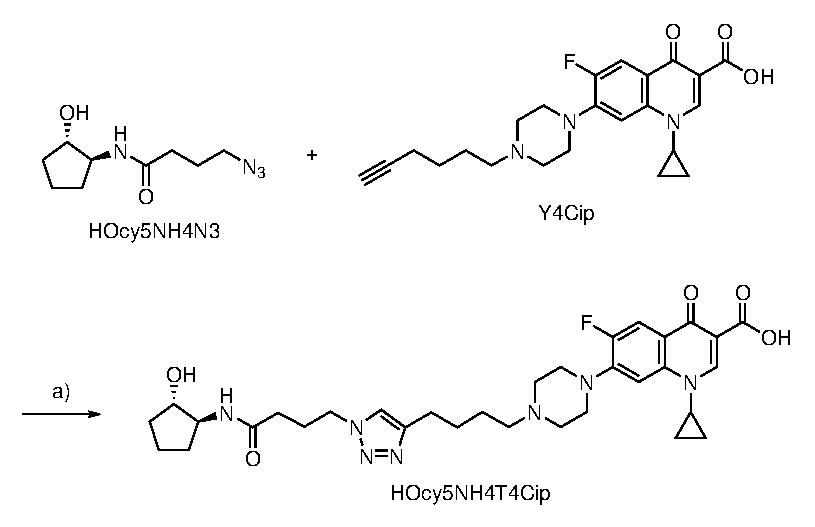
\includegraphics[scale=1]{HOcy5NH4T4Cip_RR_synth}
		\caption{\label{sch:HOcy5NH4T4Cip_RR_synth}}
	\end{center}
\end{scheme}

This worked.
